\section{Existing System: \idx{ScaleNet}} % (fold)
\label{sec:scalenet}

\idx{ScaleNet} \cite{SIE06} is a research project developed between 2005 and 2009.
Partly sponsored by the \emph{German Ministry of Education}, several major corporations participated, including \emph{Deutsche Telekom AG}, \emph{Alcatel SEL AG}, \emph{Eriksson GmbH}, \emph{Lucent Technologies} and \emph{Siemens AG}.
\ida{T-Labs} was specifically one of the departments more closely involved.

\begin{wrapfigure}{r}{0.5\textwidth}
  \centering
    
\includegraphics[width=0.48\textwidth]{logo-scalenet}
  \caption{\idx{ScaleNet} logo}
  \label{fig:logo-scalenet}
\end{wrapfigure}

The aim of \idx{ScaleNet} is to provide a \ida{NGN} that integrates different wireless and wireline access technologies.
It is advertised as a scalable, cost effective and efficient \ida{FMC} solution.

\subsection{System Overview} % (fold)
\label{sub:overviewscalenet}

\idx{ScaleNet} addresses both service and network convergence.
At the lower level, the system supports a multitude of heterogeneous physical and logical network elements of fixed and mobile networks into one single all-IP infrastructure.
Figure~\ref{fig:scalenet-structure} lists some of the protocols that could be used \cite{SIV08}.

\begin{figure}[htbp]
  \centering
    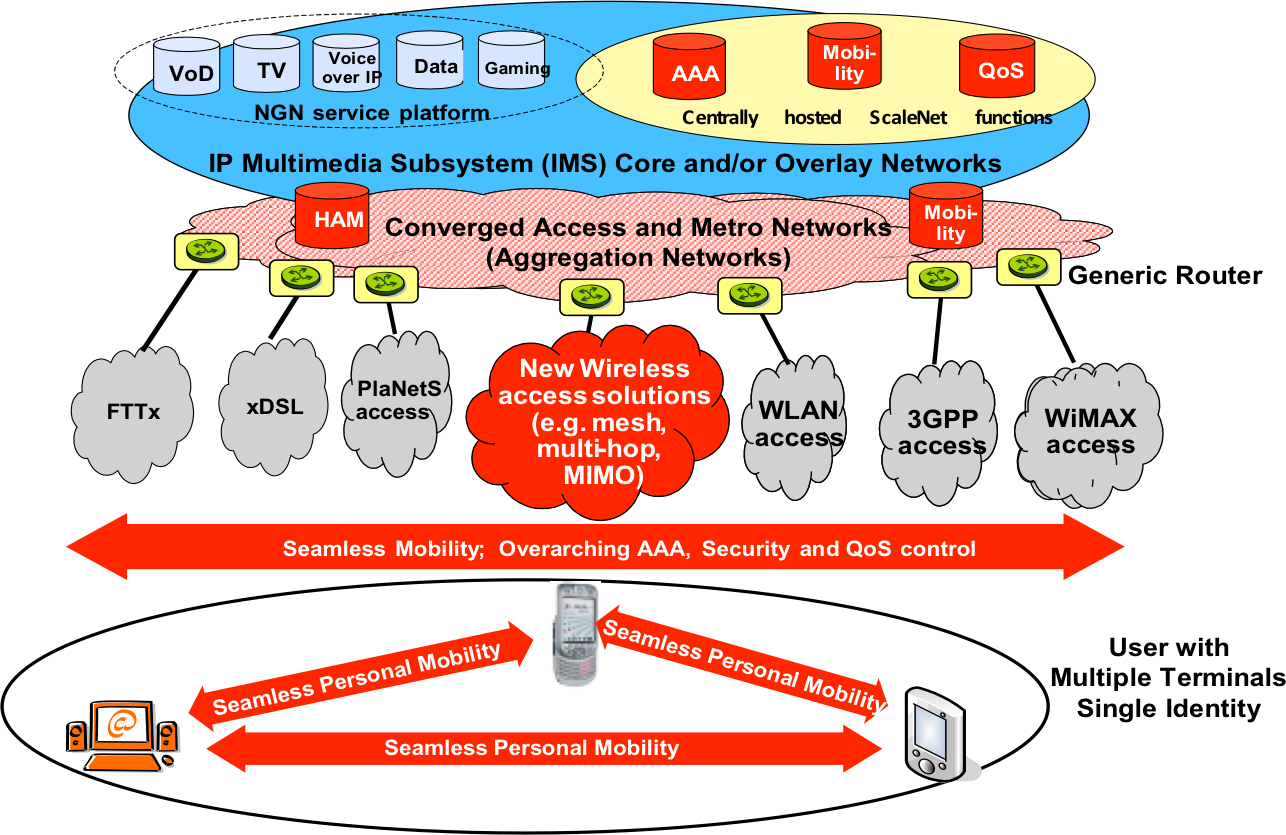
\includegraphics[width=\textwidth]{scalenet-structure}
  \caption{Structure of the system}
  \label{fig:scalenet-structure}
\end{figure}

At a upper level, multimedia services relay on the \ida{IMS} framework for the delivery.
Theoretically \idx{ScaleNet} could support other protocols like Overlay Networks or \ida{P2P}, but \ida{IMS} is the one used by the current implementation.

It is important to notice that the own network is user-centric, and transparently handles identities by using \ida{SIP}.
This eases handling users with multiple devices; therefore applications do not have to worry about that part.

It is also important to define what a session means in this system.
A session refers to the current use of a service, so for every service that the user is enjoying a session is created.
For example, if it is viewing a movie but also talking on the \ida{IP} phone, there are two sessions at the same time.

The creation of a session implies that a new service is created, but it goes the other way around too.
If a session is deleted, that service must stop.
If the user ends the service, the session must be deleted.
That means sessions have to be synchronized with the actual services.

A session is also linked to the device that the user is using.
The system allows the copy and transfer of sessions to other devices that he owns, wherever it makes sense.
Since the current implementation has also basic social capabilities, that session can also be transferred or copied to a user's contact.
In the context of this application a user's contact is called ``buddy''.
Figure~\ref{fig:scalenet-structure} lists some of the services that can be offered:

\begin{itemize}
  \item Voice \et{} Video Calls
  \item Mobile TV \et{} \ida{VOD}
  \item \index{MMOG}\acp{MMOG}
  \item Internet Access
\end{itemize}

The work described in this document is primarily focused on the second application, i.e., video streaming.
The idea is that the user can buy a video and play it anywhere using any supported device.

% subsection overviewscalenet (end)

\subsection{\idx{IMS} Demonstrator} % (fold)
\label{sub:demonstrator}

\begin{figure}[p]
  \centering
    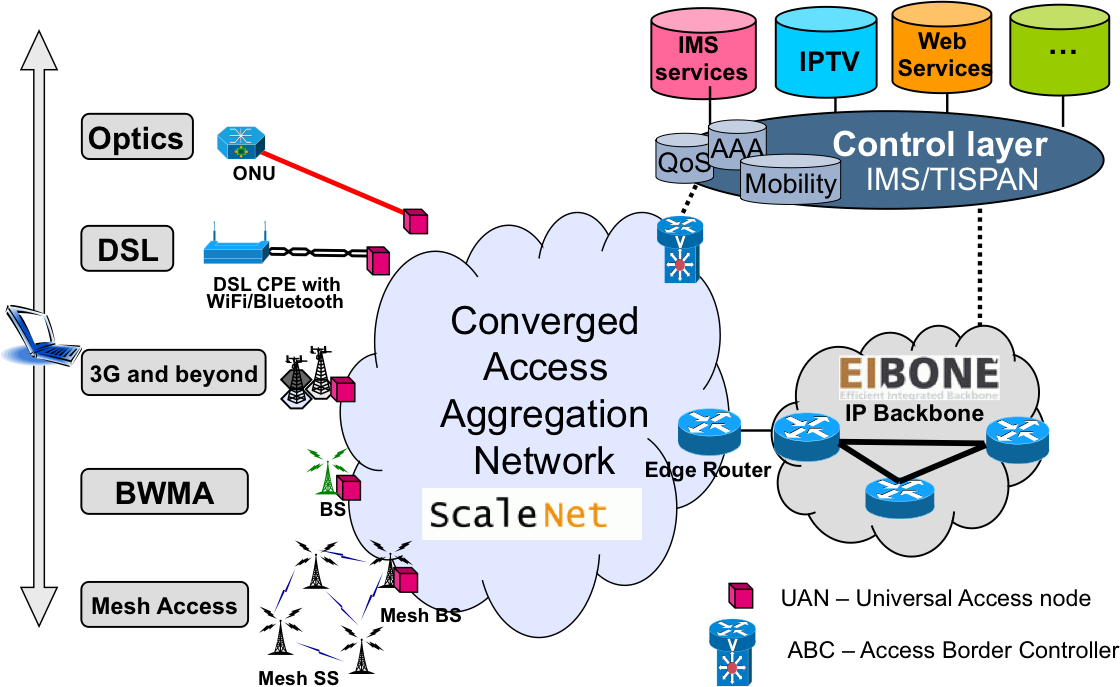
\includegraphics[width=\textwidth]{ims-arch}
  \caption{System architecture}
  \label{fig:ims-arch}
\end{figure}

\begin{figure}[p]
  \centering
    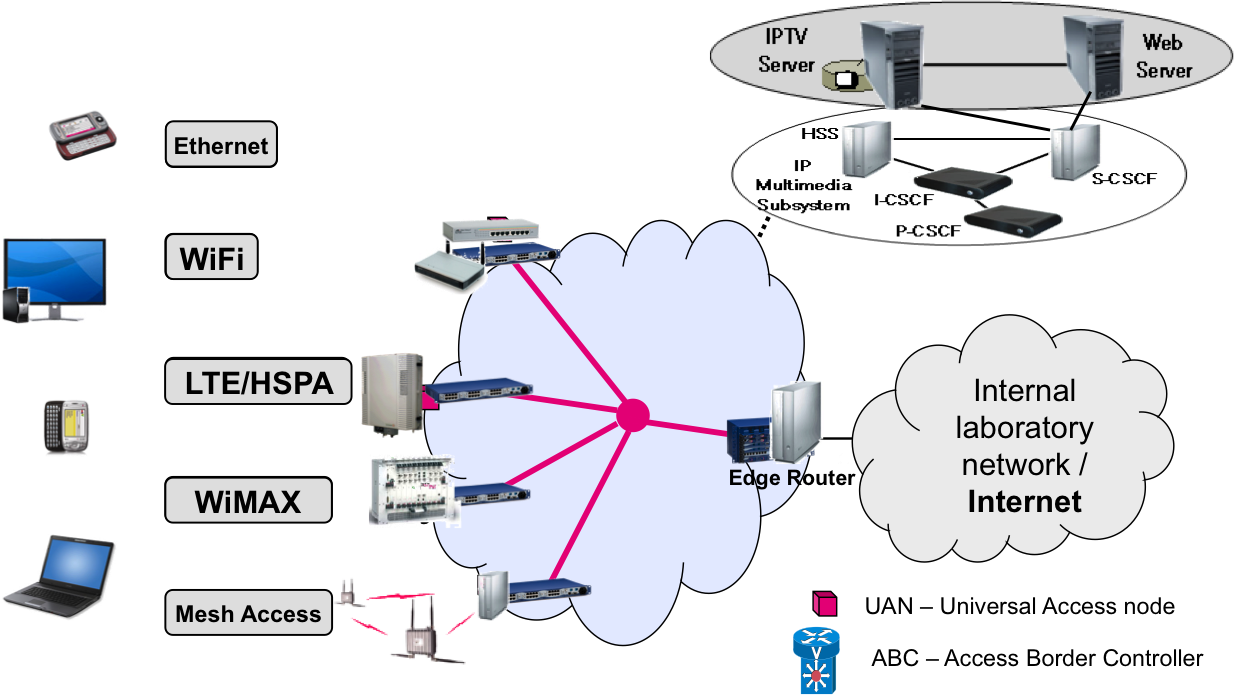
\includegraphics[width=\textwidth]{ims-arch-real}
  \caption{Architecture of the demonstrator}
  \label{fig:ims-arch-real}
\end{figure}

A logical view of the system is depicted in Figure~\ref{fig:ims-arch}, explaining the important nodes based on the capabilities needed.
The information relevant to this project is contained in the upper right corner of the figure, the nodes behind the control layer.

In the offices of \ida{T-Labs} in Berlin and Darmstadt there is a demonstrator with a working implementation of \idx{ScaleNet}.
That demonstrator is composed by several servers and a network infrastructure that enables access to the system using different network protocols and devices.
In Figure~\ref{fig:ims-arch-real} the actual network and hardware are exposed, replacing the same space as in the logical view (Figure~\ref{fig:ims-arch}).

\begin{figure}[htbp]
  \centering
    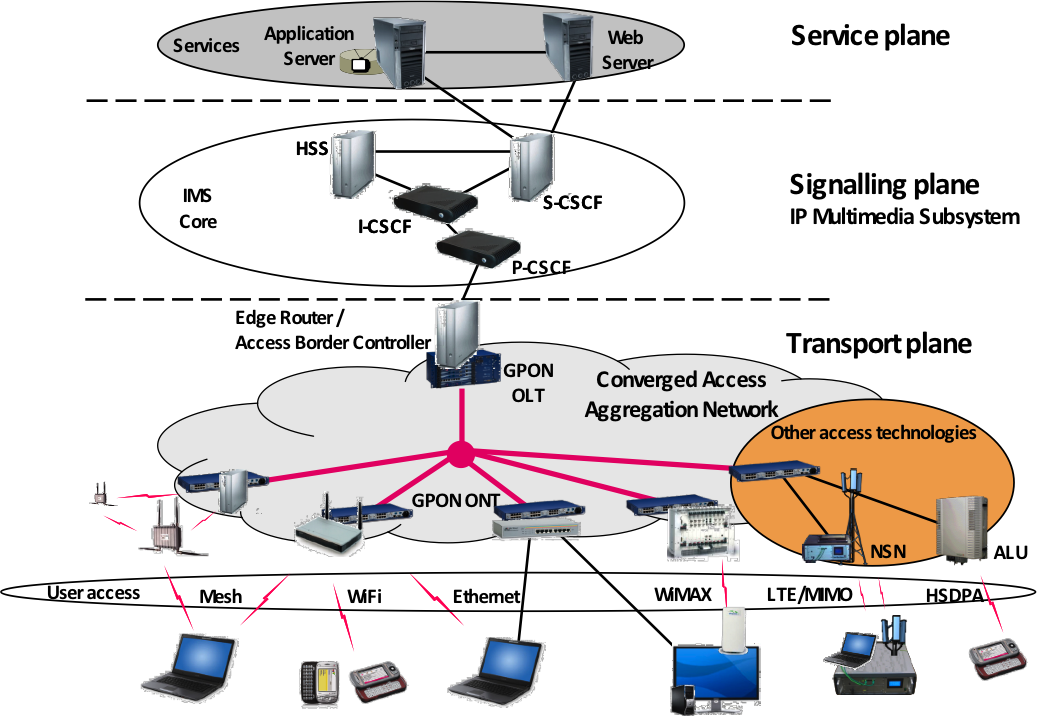
\includegraphics[width=\textwidth]{ims-setup}
  \caption{Setup of the demonstrator}
  \label{fig:ims-setup}
\end{figure}

Figure~\ref{fig:ims-setup} describes the setup in a better way and highlights the three different planes of the demonstrator.
The developed web application is executed from the \idx{Web Server} and the \idx{Application Server}, since it belongs to the service plane.
The signaling plane has also to be taken into account, because it communicates directly with the servers.

However, that is not the real deployment of the hardware used.
Whether for convenience or efficiency, tasks are distributed between two main servers.
This does not affect the logic of the system, since those tasks could be easily decoupled in an alternate deployment with more servers.
Anyway, the interesting pieces of hardware for this project are:

\begin{description}
  \item[\ida{IMS} core] This machine contains the \ida{IMS} server\footnote{The IMS core is open source software from Fraunhofer FOKUS and it can be freely downloaded from: \url{http://www.openimscore.org/}}, but since the \ida{IMS} load is not very high, it is responsible for other things.
  It acts as a \idx{Web Server} (using Apache Web Server\footnote{\url{http://httpd.apache.org/}}) serving \idas{PHP} applications.
  It is also the internal \idas{DNS} server.
  \item[\idx{Application Server}] This is the \idas{IPTV} server, where the video content is streamed.
  It is also a \idx{Web Server}, but it serves \idx{Java} applications based on the \idas{OSGi} framework\footnote{\url{http://www.osgi.org/}}.
  \item[User Devices] Devices intended for the user to access the services.
  There is a TV, a laptop and several phones.
  All of them run a custom \ida{IMS} client that holds a connection to the servers, allowing the identification and adding \idas{IPTV} and \idas{VoIP} capabilities to those devices.
  In the last phase of the development, an \idx{iPhone} was added for testing purposes.
\end{description}

This demonstrator contains several demo applications running.
The interesting one for this project is the application that handles \idas{IPTV} streaming.

% subsubsection stoppingplayback (end)

\subsection{Personal Network Administration Interface (\idx{PNAI})} % (fold)
\label{sub:pnai}

The Web interface used for the management of sessions is called \ida{PNAI}. From this interface the user can obtain this information:

\begin{itemize}
  \item All devices and registered in the system for that user and their online status.
  \item All buddies for that user and their online status.
  \item All multimedia sessions related to the user. This includes:
  \begin{itemize}
    \item The sessions running on his devices, no matter who paid for that content.
    \item The sessions running on devices from his buddies and started/paid by that user.
  \end{itemize}
\end{itemize}

Those are passive actions, but from that same view the user can initiate some operations to control the system.
In Figure~\ref{fig:usecasesiptv} all the available operations relating sessions are listed following a use case diagram.

\begin{figure}[htbp]
  \centering
    \includegraphics[width=\textwidth]{diagrams/usecases-pnai-old.1}
  \caption{Use cases for the IPTV application}
  \label{fig:usecasesiptv}
\end{figure}

In that diagram colors are used to differentiate the different kind of use cases covered. Also two visual marks (* and **) are added in case this is a copy in black a white. The meaning of the colors are explained according to this legend:

\begin{description}
  \item[Green] Available already in the main \ida{PNAI} page.
  \item[Purple (\emph{marked with *})] Available in an individual page outside of the main \ida{PNAI} page.
  \item[Red (\emph{marked with **})] Not implemented.
\end{description}

As we can see, the main \ida{PNAI} page has already a lot of functionality, but it can contain even more. Basically the actions available to that user in that page are:

\begin{itemize}
  \item Terminate a session of a user device or of a buddy if the session is owned by that user.
  \item Transfer (handover) or copy (duplication) a existing session to a user device or to a buddy if the session is owned by that user. That is, if one buddy bought the content for us, we cannot transfer again that content to another buddy.
\end{itemize}

Beside of these session related operations, there are other management operations.
For example, selecting which device is the default, adding/removing devices or adding/removing buddies.
For this document they are not relevant since they remained untouched.

Figure~\ref{fig:pnai-old} shows the old appearance of the main page for a logged user, before any work began.
On the left side of the page there is the \idx{Device List}, where the devices owned by that user are drawn.
On the right side there is the \idx{Buddy List}, where the user's buddies are listed.
Finally, the trash bin is in the lower right corner of the \idx{Device List}. 

\begin{figure}[htbp]
  \centering
    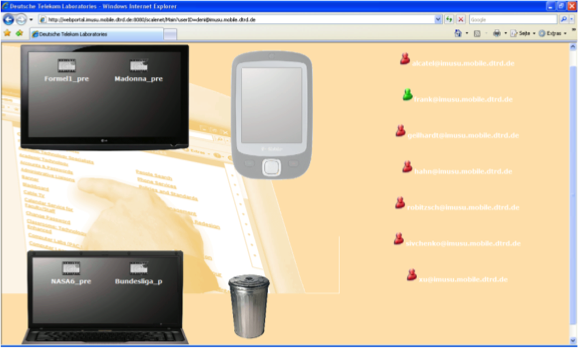
\includegraphics[width=\textwidth]{pnai-old}
  \caption{Old main \idas{PNAI} page}
  \label{fig:pnai-old}
\end{figure}

The devices that are offline are disabled and are drawn with a dimmed appearance.
The buddies that are online are preceded by a green icon, while the ones that are offline are preceded by a red icon.

Devices or buddies that are online act as session containers.
The reason for the devices to be so big is because inside them the current sessions are drawn.
Besides the name of the content playing, session have an icon that changes depending on the type of session (video, audio, call, etc).

The user can interact with the sessions through the mouse using drag\et{}drop.
For example, the user can \emph{grab} the icon he wants and drop it in another container to copy or transfer that session.
That is a very visual and fast way to manage sessions.

When a user drops the session in another container, a menu will appear to ask the user if he wants to copy or transfer that session.
The trash bin acts also as a container, but in a special way: when a session is dropped in the trash bin, that session is automatically deleted, with no menu involved.

\subsubsection{Use Cases} % (fold)
\label{ssub:usecasesold}

\begin{center}
  \begin{usecase}[Stop a session of a device]
    \label{tab:usecasestopdevice}%
    \usecaseactor{System user}
    \usecasepre{A session is already running on a device, and it is showing in the \ida{PNAI} interface inside of that device.}
    \usecasepost{Session must terminate, i.e., the content must stop playing. The user must be notified with a popup and the session icon must be deleted from the \ida{PNAI} interface.}
    \usecasemain{
      \begin{usecasepath}
        \item User starts dragging the session icon.
        \item A copy of the session icon appears under the user's cursor, and follows the cursor until the user drops it.
        \item User drops the cloned session icon into the trash.
        \item A popup appears to notify the user that the action is in progress and the cloned session icon is deleted from the view.
        \item The content stops playing.
        \item The popup disappears and the original session icon is deleted from the view.
      \end{usecasepath}
    }
    \usecasealt{1}{
      \begin{usecasepath}[b]
        \setcounter{enumi}{2}
        \item User drops the session into a blank space.
        \item Action is cancelled.
      \end{usecasepath}
    }
    \usecasealt{2}{
      \begin{usecasepath}[c]
        \setcounter{enumi}{4}
        \item There is an error with the server and the content keeps playing.
        \item The content of the popup changes to notify the user that there was an error with the server and the action could not be completed.
        After 5 seconds it disappears.
        \item Action is cancelled.
      \end{usecasepath}
    }
    \usecasealt{3}{
      \begin{usecasepath}[d]
        \item There is an error with the server and the content keeps playing.
        \item The content of the popup changes to notify the user that there was an error with the server and the action could not be completed.
        After 5 seconds it disappears.
        \item Action is cancelled.
      \end{usecasepath}
    }
  \end{usecase}
\end{center}

The use case for terminating a session that a buddy is playing and that we own is very similar:

\begin{center}
  \begin{usecase}[Stop a session of a buddy]
    \label{tab:usecasestopbuddy}%
    \usecaseactor{System user}
    \usecasepre{A session owned by the user is running on a device, and it is showing in the \ida{PNAI} interface near that buddy's name.}
    \usecasepost{Session must terminate, i.e., the content must stop playing. The user must be notified with a popup and the session icon must be deleted from the \ida{PNAI} interface. The buddy is \emph{not} notified, the content stops without warning.}
    \usecasemain{
      \begin{usecasepath}
        \item User starts dragging the session icon.
        \item A copy of the session icon appears under the user's cursor, and follows the cursor until the user drops it.
        \item User drops the cloned session icon into the trash.
        \item A popup appears to notify the user that the action is in progress and the cloned session icon is deleted from the view.
        \item The content stops playing.
        \item The popup disappears and the original session icon is deleted from the view.
      \end{usecasepath}
    }
    \usecasealt{1}{
      \begin{usecasepath}[b]
        \setcounter{enumi}{2}
        \item User drops the session into a blank space.
        \item Action is cancelled.
      \end{usecasepath}
    }
    \usecasealt{2}{
      \begin{usecasepath}[c]
        \setcounter{enumi}{4}
        \item There is an error with the server and the content keeps playing.
        \item The content of the popup changes to notify the user that there was an error with the server and the action could not be completed.
        After 5 seconds it disappears.
        \item Action is cancelled.
      \end{usecasepath}
    }
  \end{usecase}
\end{center}

% subsubsection usecasesold (end)

\subsubsection{Components} % (fold)
\label{ssub:componentsold}

As explained in \S\ref{sub:demonstrator}, the software is mainly executed in three machines: two servers and a client.
Figure~\ref{fig:componentdiagramsold} shows all the relevant components running inside those machines and how they interact with each other.

\begin{figure}[htbp]
  \centering
    \includegraphics[width=\textwidth]{diagrams/component-pnai-old.1}
  \caption{Component diagram for the old \idas{PNAI}}
  \label{fig:componentdiagramsold}
\end{figure}

That component diagram brings some interesting aspects about the system, although we are only interested in several of them:

\begin{itemize}
  \item The \idas{SIP} protocol is used for the IMS part, but this is not important for the work done, as both the server and the client were not touched.
  \item The \idas{SSCON} manages the sessions and acts as the bridge between the actual services and the web interface shown to the user.
  Actions from the web interface are notified through \idas{UDP} calls.
  \item In this diagram, though, there are two parts missing that are almost completely irrelevant for this document.
  These are the application server component that streams the content and the multimedia player installed in the user device.
  The protocols used between these two components are not interesting for us, so for sake of simplicity, they don't appear here.
  The only important thing is that the \idas{SIP} client controls the external player, so the web interface does not handle the video streaming.
  \item There are two MySQL databases in use:
  \begin{description}
    \item[\idx{HSS DB}] This is the master database, and it is always up to date.
    It contains information about the user status, his buddy list and registered devices.
    \item[\idx{Personal DB}] This is an additional database that depends on the HSS DB.
    This database gather all the information needed for the \idas{PNAI}, since it contains all the relevant information from the \idx{HSS DB} plus the session information obtained from the \idas{SSCON}.
    Periodically, the \idas{SSCON} polls information from the master database and then updates this slave database, so the information can be a bit outdated compared to the \idx{HSS DB}.
    As stated in the diagram, the \idas{OSGi} component grabs the information it needs from this database, by polling it periodically.
  \end{description}
  \item Once the page is sent to the browser, the web interface continues talking with the server through a \idas{TCP} socket without reloading the page.
  This goes both ways, since it is used for sending actions and receiving data following a push model (so no delays polling).
  Since, at the time of developing the original application, there was no way to get that using only basic web standards, it uses a \idx{Java applet} to handle the socket communications.
\end{itemize}

\begin{figure}[htbp]
  \centering
    \includegraphics[width=\textwidth]{diagrams/sequence-handover-old.1}
  \caption{Sequence diagram for the old \idas{PNAI}}
  \label{fig:handoverscenarioold}
\end{figure}

Figure~\ref{fig:handoverscenarioold} shows the flow of the application in the scenario where the user wants to transfer a session from his device to one of those buddies.
Blue lines belong to the main logical flow, while the yellow ones belong to the video streaming process.
Other usage scenarios are very similar to this one, so they are ignored since this one explains well how and when they communicate.

As we can see, the web interface (written in \idx{JavaScript}) talks back and forth with the \idx{Java applet} using simple method calls, since all the code interface are directly available between them.
Then the \idx{Java applet} translates those calls to strings with the method names and parameters and sends it to the \ida{OSGi} using the \idas{TCP} connection.

At the right part of the diagram, it is clear that the sessions are controlled using \idas{SIP} messages.
Given that \idx{ScaleNet} is a very decentralized network by design, the \idas{SSCON} delegates to the \idas{SIP} clients running in the devices all the talking with the \idx{Application Server}.

It is interesting to note that everything is mostly asynchronous, so there is not a lot of calls that block.
Therefore the use of threads and callbacks is widespread in all components.

% subsubsection componentsold (end)

\subsubsection{Personal DB} % (fold)
\label{ssub:personaldb}

The database that is directly used by the \idas{PNAI} is the \idx{Personal DB}. The most important table is the \texttt{current\_session} table, where is all the information about the sessions that are currently active.
Table~\ref{tab:sessiondb} explains all the fields in this table, and Table~\ref{tab:sessiondbexample} details an example entry.

\begin{generictable}[Current session table architecture]{2}
  {|p{0.2\textwidth}|p{0.69\textwidth}|}
  {\generictitletwo{Field name}{Description}}
  \label{tab:sessiondb}%
  \idc{id} & Identifier, auto-increment integer \\ \hline
  \idc{impi} & Private identity of user \\ \hline
  \idc{impu} & Public identity of user \\ \hline
  \idc{callid} & Unique number to identify session details \\ \hline
  \idc{partner} & Next party of session (AS identity if client to AS or impu of partner if client to client) \\ \hline
  \idc{as} & \idx{Application Server} identity (client to AS) or NULL (client to client) \\ \hline
  \idc{ip} & \idas{IP} address for impu \\ \hline
  \idc{initiator} & impu who sends the INVITE message \\ \hline
  \idc{owner} & impi who needs to pay for the session. Usually the impi who sends the INVITE message, but it can be the impi who sends the REFER message in case of transfer/duplication \\ \hline
  \idc{session\_name} & Name of the session \\ \hline
  \idc{type} & Type of the session (audio/video) \\ \hline
  \idc{bw} & Bandwidth of the session \\ \hline
  \idc{source} & \idas{URL} of the source \\ \hline
  \idc{lov} & Type of video transmission (live/video on demand/tv)\\ \hline
  \idc{cid/did/tid} & Integers related to \idas{QoS} parameters \\ \hline
  \idc{session\_flag} &
  0 if it is a normal session \newline
  1 if it is a transferred session \newline
  2 if it is a duplicated session
  \\ \hline
\end{generictable}

\begin{generictable}[Current session table example]{2}
  {|p{0.2\textwidth}|p{0.69\textwidth}|}
  {\generictitletwo{Field name}{Example value}}
  \label{tab:sessiondbexample}%
  \idc{id} & 3 \\ \hline
  \idc{impi} & deni@imusu.mobile.dtrd.de \\ \hline
  \idc{impu} & mda.deni@imusu.mobile.dtrd.de \\ \hline
  \idc{callid} & 783457644 \\ \hline
  \idc{partner} & as@imusu.mobile.dtrd.de or tv.hahn@imusu.mobile.dtrd.de \\ \hline
  \idc{as} & as@imusu.mobile.dtrd.de \\ \hline
  \idc{ip} & 19.168.5.92 \\ \hline
  \idc{initiator} & mda.deni@imusu.mobile.dtrd.de or as@imusu.mobile.dtrd.de \\ \hline
  \idc{owner} & deni@imusu.mobile.dtrd.de \\ \hline
  \idc{session\_name} & NASA \\ \hline
  \idc{type} & video \\ \hline
  \idc{bw} & 5000 \\ \hline
  \idc{source} & http://appserver:9000 \\ \hline
  \idc{lov} & video on demand/\\ \hline
  \idc{cid/did/tid} & 3/5/12 \\ \hline
  \idc{session\_flag} & 0 \\ \hline
\end{generictable}

Other important table is the \texttt{user\_status} table, that lists all the users in the system and some basic information about them.
Table~\ref{tab:userdb} explains all the fields in this table, and Table~\ref{tab:userdbexample} details an example entry.

\begin{generictable}[User status table architecture]{2}
  {|p{0.2\textwidth}|p{0.69\textwidth}|}
  {\generictitletwo{Field name}{Description}}
  \label{tab:userdb}%
  \idc{id} & Identifier, auto-increment integer \\ \hline
  \idc{impi} & Private identity of user \\ \hline
  \idc{impu} & Public identity of user \\ \hline
  \idc{impi\_id} & Unique id to identify impi \\ \hline
  \idc{impu\_id} & Unique id to identify impu \\ \hline
  \idc{status} & Status of impu: 1 (online), 0 (offline) \\ \hline
\end{generictable}

\begin{generictable}[User status table example]{2}
  {|p{0.2\textwidth}|p{0.69\textwidth}|}
  {\generictitletwo{Field name}{Example value}}
  \label{tab:userdbexample}%
  \idc{id} & 1 \\ \hline
  \idc{impi} & deni@imusu.mobile.dtrd.de \\ \hline
  \idc{impu} & laptop.deni@imusu.mobile.dtrd.de \\ \hline
  \idc{impi\_id} & 67 \\ \hline
  \idc{impu\_id} & 35 \\ \hline
  \idc{status} & 1 \\ \hline
\end{generictable}

Finally, there is a third table that handles the relationships between friends called \texttt{buddy\_list}.
It is a very simple table modeling a classic many-to-many relationship, but anyway Table~\ref{tab:buddydb} explains all its fields, and Table~\ref{tab:buddydbexample} details an example entry.

\begin{generictable}[Buddy list table architecture]{2}
  {|p{0.2\textwidth}|p{0.69\textwidth}|}
  {\generictitletwo{Field name}{Description}}
  \label{tab:buddydb}%
  \idc{id} & Identifier, auto-increment integer \\ \hline
  \idc{impi\_id} & Unique id to identify impi (identical to impi\_id of \texttt{user\_status} table) \\ \hline
  \idc{buddy\_impi\_id} & Unique id to identify the buddy impi \\ \hline
\end{generictable}

\begin{generictable}[Buddy list table example]{2}
  {|p{0.2\textwidth}|p{0.69\textwidth}|}
  {\generictitletwo{Field name}{Example value}}
  \label{tab:buddydbexample}%
  \idc{id} & 2 \\ \hline
  \idc{impi\_id} & 56 \\ \hline
  \idc{buddy\_impi\_id} & 67 \\ \hline
\end{generictable}

These tables are not changed during the development explained in this document, neither the software that access those tables directly.
However, it is interesting to know the kind of data they have because indirectly it is the same data we are going to process.

% subsubsection personaldb (end)

\subsubsection{Messages} % (fold)
\label{ssub:messagesold}

Of all the messages sent inside the system, the most important ones for us are sent though the \idas{TCP} socket.
These are processed and generated by the web interface and the \idas{OSGi} backend, but they follow a different format depending which component sends the message.

Messages generated by the backend consist of serialized objects following a very simple format.
There are three kind of data objects that can be sent over the wire: devices, buddies and sessions.

A serialized object is a string that starts with the type of the object (\texttt{device}, \texttt{buddy}, \texttt{session}), followed by the vertical bar character `|' as delimiter.
Then the attributes for that object are appended one by one, separated by the same delimiter.
If the values are not strings, they are converted directly, for example a boolean with value \texttt{true} will be passed as the string \texttt{"true"}.

The client does not know when a transfer or duplication happens, it is only notified of creation and deletion of things.
For example, as seen in the Figure~\ref{fig:handoverscenarioold}, when a transfer happens the interface received two commands, first creating a new session and then deleting the original session.

To notify that a new object needs to be created in the view, the backend just sends the serialized object, without adding anything else.
To notify that an existing object has to be deleted from the view, the string is the same but preceded by the text \texttt{"deleted|"} (that is, \emph{deleted} and the delimiter).

Table~\ref{tab:notificationsexamples} comprises all the different messages that can be sent from the \idas{OSGi} backend to the \idx{Java applet} with examples.

\begin{generictable}[Format of the notifications sent to the applet]{2}
  {|p{0.2\textwidth}|p{0.69\textwidth}|}
  {\generictitletwo{Notification}{Format \et{} Example}}
  \label{tab:notificationsexamples}%
  Create/update device & \texttt{device|\emph{impi}|\emph{impu}|\emph{online}} \newline
    \texttt{device|hahn@imusu.mobile.dtrd.de\newline
    $\hookrightarrow$|tv.hahn@imusu.mobile.drtd.de|true} \\ \hline
  Delete device & \texttt{deleted|device|\emph{impi}|\emph{impu}|%
    \emph{online}} \newline
    \texttt{deleted|device|hahn@imusu.mobile.dtrd.de\newline
    $\hookrightarrow$|tv.hahn@imusu.mobile.drtd.de|false} \\ \hline
  Create/update buddy & \texttt{buddy|\emph{id}|\emph{name}|\emph{online}}%
    \newline
    \texttt{buddy|3|hahn@imusu.mobile.dtrd.de|false} \\ \hline
  Delete buddy & \texttt{deleted|buddy|\emph{id}|\emph{name}|\emph{online}}%
    \newline
    \texttt{deleted|buddy|3|hahn@imusu.mobile.dtrd.de\newline
    $\hookrightarrow$|false} \\ \hline
  Create/update session & \texttt{session|\emph{id}|\emph{type}|\emph{name}%
    |\emph{owner}|\emph{initiator}|\emph{impi}\newline
    $\hookrightarrow$|\emph{impu}|\emph{icon}}
    \newline
    \texttt{session|3|video|NASA\newline
    $\hookrightarrow$|hahn@imusu.mobile.dtrd.de\newline
    $\hookrightarrow$|hahn@imusu.mobile.dtrd.de\newline
    $\hookrightarrow$|hahn@imusu.mobile.dtrd.de\newline
    $\hookrightarrow$|laptop.hahn@imusu.mobile.dtrd.de\newline
    $\hookrightarrow$|http://imusu.mobile.dtrd.de/img/icon.png} \\ \hline
  Delete session & \texttt{deleted|session|\emph{id}|\emph{type}|\emph{name}%
    |\emph{owner}\newline
    $\hookrightarrow$|\emph{initiator}|\emph{impi}|\emph{impu}|\emph{icon}}
    \newline
    \texttt{deleted|session|3|video|NASA\newline
    $\hookrightarrow$|hahn@imusu.mobile.dtrd.de\newline
    $\hookrightarrow$|hahn@imusu.mobile.dtrd.de\newline
    $\hookrightarrow$|hahn@imusu.mobile.dtrd.de\newline
    $\hookrightarrow$|laptop.hahn@imusu.mobile.dtrd.de\newline
    $\hookrightarrow$|http://imusu.mobile.dtrd.de/img/icon.png} \\ \hline
\end{generictable}

% subsubsection messagesold (end)

\subsubsection{Class Diagrams} % (fold)
\label{ssub:classdiagramsold}

\begin{figure}[htbp]
  \centering
    \includegraphics[width=\textwidth]{diagrams/class-pnai-js-old.1}
  \caption{Class diagram for the old \idas{PNAI}}
  \label{fig:classdiagramsold}
\end{figure}

% subsubsection classdiagramsold (end)
% subsection pnai (end)
% section scalenet (end)